\chapter{Results}\label{chapter:results}

\section{Statistical Methodology}\label{sec:statisticalModel}
The calculation of cross section and statistical significances were made using Higgs Analysis Combined Limit (\combine) tool~\cite{Combine}, which is based on the RooStats package~\cite{Moneta:2010pm,Schott:2012zb}.
The \combine tool is used to determine the signal strength using a binned Maximum Likelihood Fit (MLF) and the significances using using an asymptotic approximation~\cite{AsymptoticFormulae}, using the Asimov dataset.

The 


\begin{equation}
L = \prod\limits_{i=1}^{\N} _{i} \frac{•}{•} \;
\label{eq:poissonLikelihood}
\end{equation}

\begin{equation}
\mathcal{L} = - L = \sum\limits_{i=1}^{\N} _{i} \frac{•}{•} \;
\label{eq:minLogLikelihood}
\end{equation}

In the following section the signal and background yields are referred to as $s$ and $b$ respectively, where both represent event counts in the probability distribution function bins.
The uncertainties for the simulated 

All the systematic uncertainties were incorporated into the fit as nuisance parameters.
The normalisation uncertainties are incorporated into the fit as log-normal nuisance parameters

Morphing for shapes

Significia

 
The fit was performed on the two channels simultaneously. 
Most systematics were assumed to be 100\% correlated between channels.

\subsection{Confidence Levels Method}\label{subsec:CLs}
The modified classical frequentist methods are  

\subsection{Data-driven background normalisation}\label{subsec:combineNormalisation}
floating in the fit



\section{Impact of the Systematic Uncertainties}\label{sec:uncertainitiesImpact}
The effect of each of the sources of systematic uncertainty considered in terms of the pull ($\frac{ \hat{\theta} - \theta_{0} }{\Delta \theta}$) and the postfit impact of varying the sources of uncertainty by $\pm 1 \sigma$ are shown in figure~\ref{fig:systematicsPull}.

\editComment{Remark on the lumi, jer are the largest uncerts and how the rest of the experimental uncerts are considerably smaller}

\begin{figure}[htbp]
\begin{center}
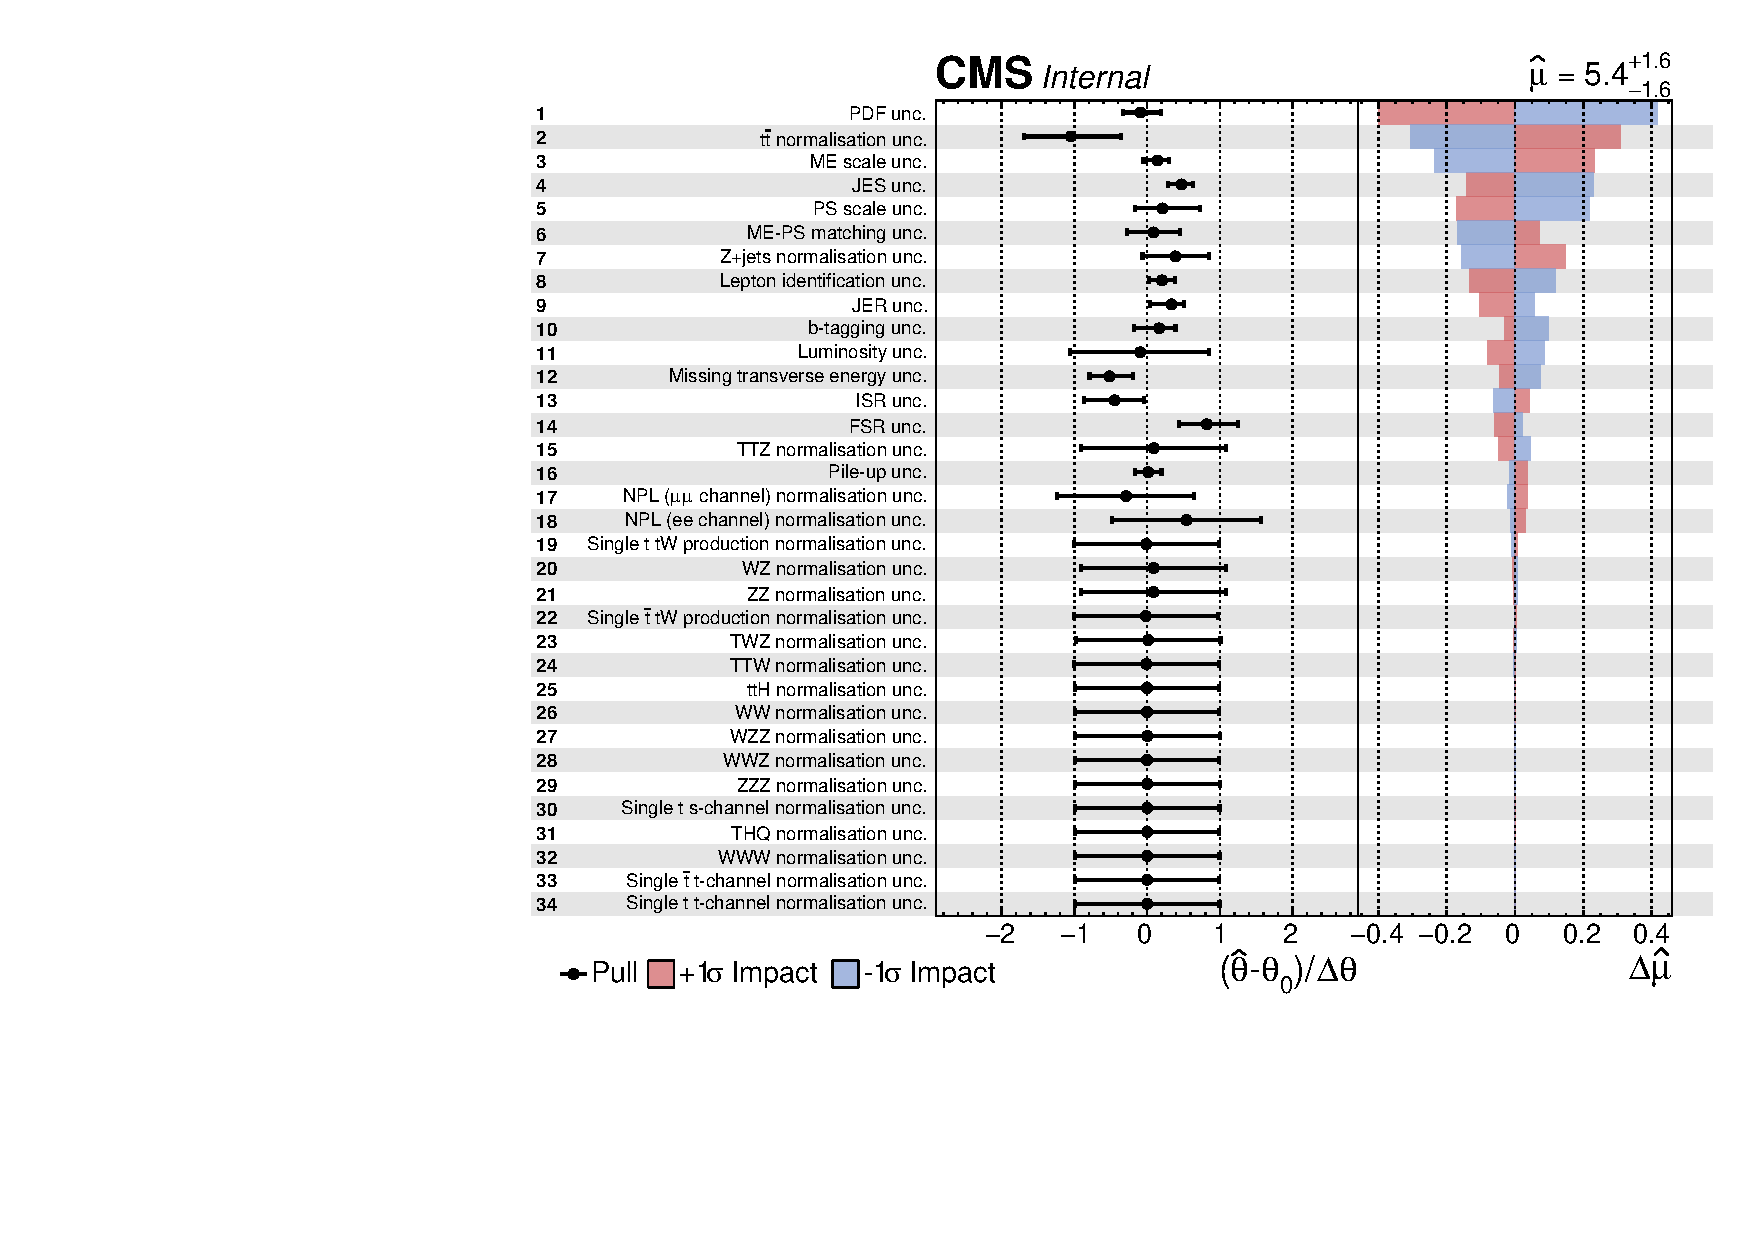
\includegraphics[width=0.97\textwidth]{figs/results/systematicsImpact.pdf}
\caption{The impact of each of the systematic uncertainties considered on the measurement made.}
\label{fig:systematicsPull}
\end{center}
\end{figure}

\section{Cross section extraction}
The cross section is 


By performing a simultaneous fit of the BDT discriminant distribution for the background-enriched sample and the BDT discriminant in the signal sample, any events in excess of the background-only hypothesis will be determined.

This excess can then be compared to the SM expectation for tZq production in order to calculate the observed signal strength and measure the cross section.

A measured signal strength of 0.0 would correspond to an observation of the background-only hypothesis alone, whilst 1.0 is the SM expectation for tZq sproduction.

\section{Signal strength significance}
The observed signal strengths, measured cross sections, and corresponding significances for the individual channels and the channels combined in the signal region using pseudo data, are shown in Table~\ref{tab:shapetxs}. 
These are [IN AGREEMENT / NOT IN AGREEMENT] with the SM cross section of  $X^{+Y}_{-Z}$.
 
\begin{table}[!h]
   \centering
   \caption{The observed signal strengths and corresponding cross sections for
   the individual channels and the channels combined at the 95\% CL.}
   \begin{tabular}{cccc}
       \hline
       Channel & $ee$ & $\mu\mu$ & \textbf{combination} \\
        \hline
        % \multicolumn{4}{c}{\combine{}} \\
        % \hline
        Signal strength & $X_{-Z}^{+Y}$ & $X_{-Z}^{+Y}$ & $X_{-Z}^{+Y}$ \\
       Cross section (fb) & $X_{-Z}^{+Y}$ & $X_{-Z}^{+Y}$ & $X_{-Z}^{+Y}$ \\
       Significance (expected) & $X_{-Z}^{+Y}$ & $X_{-Z}^{+Y}$ & $X_{-Z}^{+Y}$ \\
       Significance (observed) & $X_{-Z}^{+Y}$ & $X_{-Z}^{+Y}$ & $X_{-Z}^{+Y}$ \\
        \hline
        % \multicolumn{4}{c}{\textsc{Theta}} \\
        % \hline
        % Signal strength & $X_{-Z}^{+Y}$ & $X_{-Z}^{+Y}$ & $X_{-Z}^{+Y}$ \\
        % Cross section (fb) & $X_{-Z}^{+Y}$ & $X_{-Z}^{+Y}$ & $X_{-Z}^{+Y}$ \\
        % Significance (expected) & $X_{-Z}^{+Y}$ & $X_{-Z}^{+Y}$ & $X_{-Z}^{+Y}$ \\
        % Significance (observed) & $X_{-Z}^{+Y}$ & $X_{-Z}^{+Y}$ & $X_{-Z}^{+Y}$ \\
        % \hline
    \end{tabular}
   \label{tab:shapetxs}
\end{table}


\section{Interpretation of the results}

\section{Other results from the Large Hadron Collider}
The search for a singly produced top in association with a Z boson in the dilepton final state presented is the first one made at the LHC and follows in the footsteps of the searches for the trilepton final state at $\sqrt{8}$ and $\sqrt{13}$ using data collected by the CMS experiment in 2012 and 2016 respectively.

Despite the dilepton final state having a larger cross section than the trilepton final state, the different final state topology makes it much more difficult to isolate the signal process.
Consequently, the \editComment{expected/observed} significance of $A$ is smaller than the significances observed for the trilepton final state by CMS~\cite{Sirunyan:2017nbr} and ATLAS~\cite{Aaboud:2017ylb} at $\sqrt{13}$.
